\section{\Acrlong{sispo}}

\gls{sispo} is a software package developed in python. It is separated in different sub-packages. The two main sub-packages are the \textit{sim} and the \textit{reconstruction} package. The third sub-package provides several image compression algorithms to test effects on reconstruction.

The software package is hosted on GitHub using a git version control system. Furthermore, the GitHub project management tools are used, including automated KanBan based projects, issue tracking and pull requests.

The most important python dependencies of \gls{sispo} are:
\begin{itemize}
    \item astropy: Astronomy package developed by \cite{robitaille2013astropy} and \cite{price2018astropy}
    \item Blender: 3D creation suite
    \item numpy: Scientific computing for python
    \item opencv: Computer vision library used for image processing
    \item OpenEXR: \gls{hdr} image reading and writing
    \item Orekit: Space dynamics library
\end{itemize}

It was attempted to reduce dependencies to other libraries as much as possible. Originally, both \textit{scikit-image} and \textit{opencv} were used. After a small benchmark between the two libraries, it was evident that \textit{opencv} performs three to seven times faster compared to \textit{scikit-image}. Hence \textit{scikit-image} was completely replaced with equivalent \textit{opencv} functions. Additionally, it was attempted to use the \textit{opencv} package to replace the \textit{OpenEXR} dependency since it is not easy to install. However, this is currently not possible as the \textit{OpenEXR} implementation of \textit{opencv} does not provide an alpha channel and is generally less flexible.

To ease development, numerous parameters are silently assigned default values if not provided e.g. for an instrument. Therefore, all parameters should be explicitly set when before running a simulation.



\subsection{User Interface}
The sispo package can be installed using pip and the GitHub project. If done, it will be installed into the site-packages folder of the used python environment. Additionally, an executable is installed, providing a \gls{cli} as user interface. The most recent possible input arguments are documented in the repository or by using the --help input. The most important arguments for the \gls{cli} are seen in Table \ref{tab:cli_args}.

\begin{table}[htpb]
\caption{Input arguments for sispo \gls{cli}}
\begin{tabular}{llll}
\hline
\textbf{Name}                            & \textbf{Variable Name} & \textbf{Default Value}     & \textbf{Description}                                                                                                      \\ \hline
\multicolumn{1}{l|}{--help}              &                        & ---                        & Prints list of arguments with hints                                                                                       \\
\multicolumn{1}{l|}{-i}                  & i                      & data/input/definition.json & Path to a definition file that defines the settings                                                                 \\
\multicolumn{1}{l|}{-v}                  & v                      & False                      & Verbose output, logging information will also be displayed on STDOUT                                                      \\
\multicolumn{1}{l|}{--cli}               & cli                    & False                      & If the \gls{cli} flag is set, an interactive \gls{cli} will be started. NOT IMPLEMENTED. \\
\multicolumn{1}{l|}{--profile}           & profile                & False                      & If the profile flag is set, Python's cProfile will be used to profile \gls{sispo} execution              \\
\multicolumn{1}{l|}{--no-sim}            & with\_sim              & True                       & If flag is set, simulation step will be skipped                                                                           \\
\multicolumn{1}{l|}{--no-render}         & with\_render           & True                       & If flag is set, rendering step will be skipped                                                                            \\
\multicolumn{1}{l|}{--no-compression}    & with\_compression      & True                       & If flag is set, compression step will be skipped                                                                          \\
\multicolumn{1}{l|}{--no-reconstruction} & with\_reconstruction   & True                       & If flag is set, reconstruction step will be skipped                                                                       \\
\multicolumn{1}{l|}{--sim-only}          & sim\_only              & False                      & If flag is set, only simulation step will be done                                                                         \\
\multicolumn{1}{l|}{--sim-render-only}   & sim\_render\_only      & False                      & If flag is set, only simulation and rendering will be done                                                                \\
\multicolumn{1}{l|}{--render-only}       & render\_only           & False                      & If flag is set, only rendering will be done                                                                               \\
\multicolumn{1}{l|}{--compress-only}     & compress\_only         & False                      & If flag is set, only compression will be done                                                                             \\
\multicolumn{1}{l|}{--reconstruct-only}  & reconstruct\_only      & False                      & If flag is set, only reconstruction will be done                                                                         

\end{tabular}
\label{tab:cli_args}
\end{table}

\gls{sispo} can be imported as a Python module. 

\subsection{Simulation Module}
The simulation module creates photo-realistic images by simulating a realistic trajectory of a \gls{sssb} and a spacecraft using orekit. This trajectory and attitude data is then used to render four images per frame, one containing only the \gls{sssb}, one where the view is kept at a constant distance from the \gls{sssb}, one calibration reference image and one that renders a realistic star background using the \gls{ucac4}. These images are composed to one image using photometry to calibrate the absolute light intensity of the different images in terms of realistic photon fluxes using the Johnson magnitude system \cite{bessel1979ubvri}.

All images during the rendering and calibration process use \gls{hdr} images to minimise the loss of information in intermediate steps.

\subsubsection{Composition}


\subsection{Compression Module}
The compression module provides compression and decompression algorithms. These can be tested against different mission scenarios and image series to investigate the impact of compression and decompression on the science quality.

The following set of compression algorithms 

\subsection{Reconstruction Module}
The reconstruction module can be used to generate a 3D model of an object using a series of images. It provides a full Multi-View Stereo reconstruction data process pipeline. To achieve this, two libraries are used and combined and called using python. The first library is \gls{omvg} by \cite{openMVG}. The second library is \gls{omvs}. 
The common steps for the complete pipeline is comprised of the following steps:
\begin{enumerate}
    \item Read in images [ImageListing in \gls{omvg}]
    \item Compute visual features [ComputeFeatures in \gls{omvg}]
    \item Match computed features between different images [MatchFeatures in \gls{omvg}]
    \item Generate point cloud from matched features [IncrementalSfM in \gls{omvg}]
    \item Export to \gls{omvs} format [openMVG2openMVS in \gls{omvg}]
    \item Increase number of points in point cloud [DensifyPointCloud in \gls{omvs}]
    \item Create a mesh from the point cloud [ReconstructMesh in \gls{omvs}]
    \item Refine the generated mesh [RefineMesh in \gls{omvs}]
    \item Apply texture to mesh to create final 3D model [TextureMesh in \gls{omvs}]
\end{enumerate}

\subsection{Setup}
\gls{sispo} can be setup with Linux and Windows. The default case used in this description is a Windows setup. Known differences or problems under Linux will be pointed out as well. While it should be possible to use a plain Python environment and pip, a miniconda environment manager was used for development. Also a C compiler is necessary. Linux has the GCC already installed, for Windows it is easiest to install Microsoft Visual Studio with \gls{msvc} and \gls{msbuild}. Another possibility when using Windows is to use vcpkg\footnote{Found at \url{https://github.com/microsoft/vcpkg}}. However, previously the openMVG and openMVS ports in vcpkg did not work. Vcpkg can also be used with Linux. However during an attempt, there were unsolvable problems when using vcpkg so everything was installed natively.
For \gls{omvg}, \gls{omvs} and star\_cats it is necessary to have the executables in the correct folder for \gls{sispo} to function. \newline

\begin{figure}
    \dirtree{%
.1 sispo.
.2 build.
.2 data.
.3 UCAC4.
.4 u4b.
.4 u4i.
.3 sensor\_database.
.3 models.
.3 input.
.2 doc.
.2 sispo.
.3 sim.
.3 compression.
.3 reconstruction.
.2 software.
.3 miniconda.
.3 vcpkg.
.3 blender.
.3 openMVG.
.4 openMVG.
.4 build\_openMVG.
.5 install.
.3 openMVS.
.4 openMVS.
.4 build\_openMVS.
.5 install.
.3 star\_cats.
.4 star\_cats.
.4 build\_star\_cats.
}
    \caption{Directory structure after setup}
    \label{fig:dir_tree}
\end{figure}
Figure \ref{fig:dir_tree} shows the assumed overall folder structure after installation. No subfolders of the build folder or any files are depicted. 

To make \gls{sispo} perform well, it is beneficial to install Nvidia CUDA Toolkit (https://developer.nvidia.com/cuda-downloads) in case an Nvidia graphics card is available.

\begin{enumerate}
    \item Clone the GitHub repository onto the local machine \\ \shellcmd{git clone https://github.com/YgabrielsY/sispo.git}. The project provides a software folder which is intended to be used to install all following software.
    \item Setup (conda) environment with dependencies (to software/miniconda folder):
    \begin{enumerate}
        \item orekit 9.3.1, the current version 10.0 have issues when once attempted. Also orekit needs a data package to function, it is distributed with \gls{sispo} in the sim module folder.
        \item astropy
        \item opencv
        \item OpenEXR\footnote{For Windows the pre-compiled package found at \url{https://www.lfd.uci.edu/~gohlke/pythonlibs/\#openexr} needs to be used because the pip or conda version do not work.}
        \item numpy
        \item Python\footnote{During development Python version 3.7 was used.}
    \end{enumerate}{}
    \item (Especially Windows) Install vcpkg to software/vcpkg folder, follow instructions at \url{https://github.com/microsoft/vcpkg}
    \item Install Blender as a python module (bpy)\footnote{During development Blender version 2.8 was used.}
    \begin{enumerate}
        \item Clone Blender git repository to software/blender/blender \\ \shellcmd{git clone git://git.blender.org/blender.git}
        \item Compile target bpy \shellcmd{make bpy}, this works also for Windows through the make.bat file provided with Blender
        \item When available: Activate CUDA in the cmake project and recompile
        \item Install bpy to python environment\footnote{Follow these instructions \url{https://blender.stackexchange.com/questions/117200/how-to-build-blender-as-a-python-module}}
    \end{enumerate}{}
    \item Install OpenMVG, follow instructions at \\ \url{https://github.com/openMVG/openMVG/blob/master/BUILD.md} or look for hints in the OpenMVG install script in the build folder.
    \begin{enumerate}
        \item Install dependencies according to instructions
        \item Clone OpenMVG GitHub repository to software/openMVG/openMVG \shellcmd{git clone --recursive https://github.com/openMVG/openMVG.git}
        \item Build to software/openMVG/build\_openMVG folder
        \item Install to software/openMVG/build\_openMVG/install folder
    \end{enumerate}
    \item Install OpenMVS, follow instructions at \\ \url{https://github.com/cdcseacave/openMVS/wiki/Building} or look at the OpenMVS install script in the build folder for hints.
    \begin{enumerate}
        \item Install dependencies according to instructions
        \item Clone OpenMVS GitHub repository to software/openMVS/openMVS \shellcmd{git clone https://github.com/cdcseacave/openMVS.git}
        \item Build to software/openMVS/build\_openMVS folder
        \item Install to software/openMVS/build\_openMVS/install folder
    \end{enumerate}
    \item Install star\_cats
    \begin{enumerate}
        \item Clone star\_cats GitHub repository to software/star\_cats/star\_cats \\ \shellcmd{git clone https://github.com/Bill-Gray/star\_cats.git}
        \item Build to software/star\_cats/build\_star\_cats \shellcmd{make}
    \end{enumerate}
    \item Download UCAC4 star catalog to data/UCAC4, use either:
    \begin{enumerate}
        \item the build/data/download\_ucac4.sh script
        \item download the folder u4b and u4i directly from \\ \url{http://casdc.china-vo.org/mirror/UCAC/UCAC4/}
    \end{enumerate}
\end{enumerate}{}

\subsection{Performance}
\subsubsection{skimage vs opencv}
The original simulation used the \gls{skimage} and OpenCV library. In order to reduce the number of dependencies, it was decided to benchmark relevant functions of the two libraries. For this comparison, OpenCV functions were used to create the same behaviour as the respective \gls{skimage} function. The benchmark compares the performance of the Gaussian filter and a special case of image resizing using local means.

Two machines were used for the benchmark to eliminate platform dependency, one running a Linux distribution and one running Windows 10.

\begin{figure}[htb]
    \centering
    \begin{subfigure}[b]{0.47\textwidth}
        \centering
        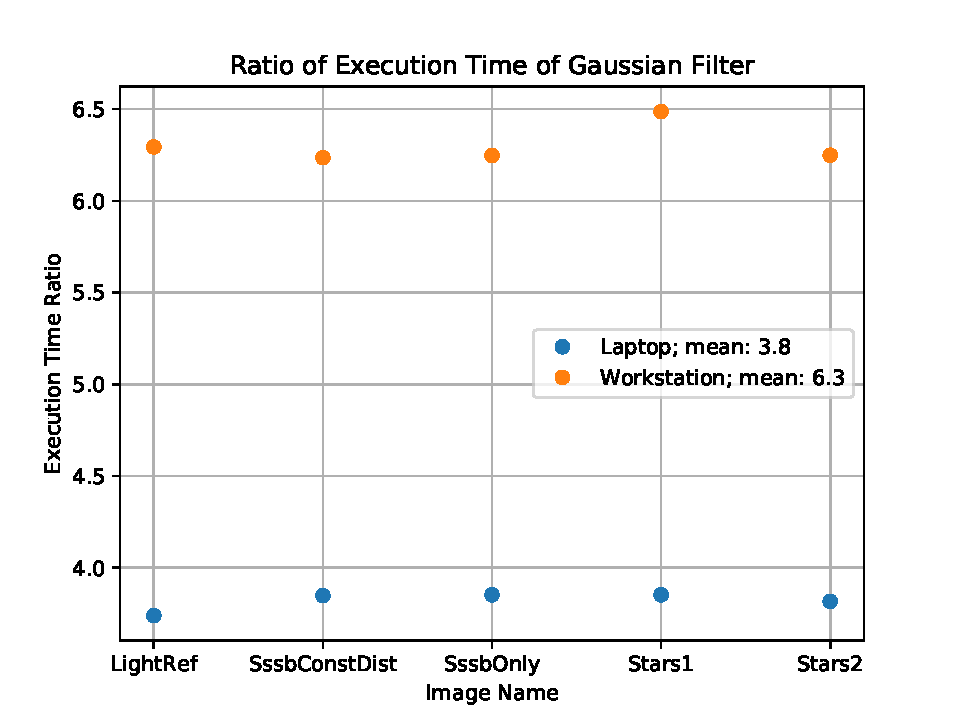
\includegraphics[width=\textwidth]{doc/thesis/0_figures/Comparison_Gaussian}
        \caption{Gaussian filtering.}
        \label{fig:bm_comparison_gauss}
    \end{subfigure}
    \begin{subfigure}[b]{0.47\textwidth}
        \centering
        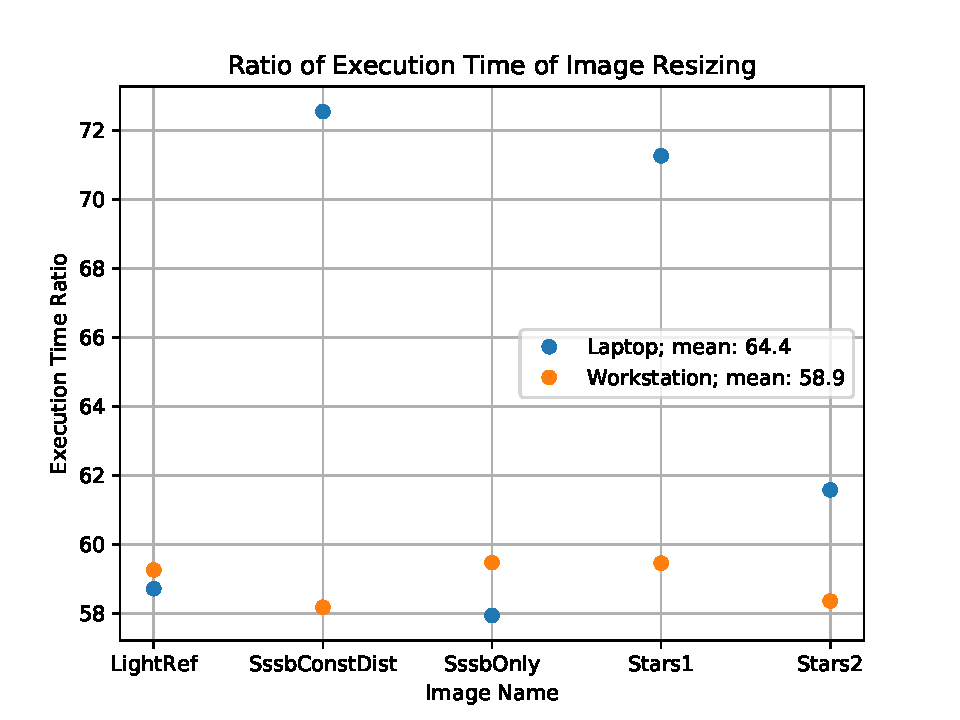
\includegraphics[width=\textwidth]{doc/thesis/0_figures/Comparison_Resize}
        \caption{Resizing.}
        \label{fig:bm_comparison_res}
    \end{subfigure}
    \caption{Comparison of execution time ratios of Gaussian filtering and resizing 5 images using OpenCV and \gls{skimage} on different computers.}
    \label{liitekuva}
\end{figure}

Maximum error gauss:  1.4864218655930017e-06
Maximum error resize:  7.152557373046875e-07

For our case, OpenCV has a clear performance advantage over the \gls{skimage} library hence only OpenCV is being used.

In addition to the performance advantages, OpenCV might be used in the future to also replace the OpenEXR depdency, if OpenCV's exr implementation is improved.

\subsection{Future Developments}
There are several issues left open within the \gls{sispo} software package. First, there is currently no realistic model of spacecraft attitude motion and control implemented. The camera of the simulation environment is perfectly oriented towards the centre of the \gls{sssb}'s nucleus during the entire simulation. Realistic rotation should cover at least two effects, motion blur due to instantaneous rotation velocities of spacecraft and off-centre pointing due to control inaccuracies. Furthermore, it is necessary to include  image distortions such as astigmatism, bokeh, coma, field curvature, glare. Moreover, it is necessary to include a gas and dust environment around the nucleus. From a technical perspective, a proper simulation of the data transmission should be included. For example, a realistic simulation for packet loss. The ultimate goal is to develop a prioritisation algorithm for the images which should prioritise data transmission on packet level.
Furthermore, the shader used to create the \gls{sssb} models should be developed further. The interface for it should be included into \gls{sispo} and restricted to values that create reasonable shaped outputs.


THOUGHTS:
-default data set, different compression and reconstruction
    -compressions: png, jpg2000 quality 1000, jpg2000 quality 500, jpg2000 quality 100, jpg2000 quality 10
-different trajectories: default : 400 km, 100km, 1000km
-different lighting situations
-different models